\documentclass[11pt]{article}

% ACL style file (https://github.com/acl-org/acl-style-files).
% Final / camera-ready version: load the style with no option.
% Use \usepackage[review]{acl} for anonymous submission or
% \usepackage[preprint]{acl} for a non-anonymous preprint with page numbers.
\usepackage[final]{acl}

% Standard package includes recommended by the ACL template
\usepackage{times}
\usepackage{latexsym}
\usepackage[T1]{fontenc}
\usepackage[utf8]{inputenc}
\usepackage{microtype}
\usepackage{inconsolata}
\usepackage{graphicx}

% Project-specific packages
\usepackage{amsmath, amssymb}
\usepackage{xcolor}
\usepackage{cleveref} % must be loaded after hyperref, which acl.sty provides

% ACL convention: capitalised cross-reference names
\crefname{section}{Section}{Sections}
\crefname{subsection}{Section}{Sections}
\crefname{appendix}{Appendix}{Appendices}
\crefname{table}{Table}{Tables}
\crefname{figure}{Figure}{Figures}
\crefname{equation}{Equation}{Equations}

\title{Orthographic, Phonetic, and Socio-Geographic Similarity of Philippine Languages}

\author{
  \textbf{Clarence Ang} \quad
  \textbf{Clive Ang} \quad
  \textbf{Roan Campo} \quad
  \textbf{Zhean Ganituen} \\
  De La Salle University\\
  2401 Taft Ave, Malate, Manila, Philippines\\
  \small{
    \texttt{\{clarence\_ivan\_ang, clive\_jarel\_c\_ang, roan\_campo, zhean\_robby\_ganituen\}@dlsu.edu.ph}
  }
}

\begin{document}
\maketitle

\begin{abstract}
  We measure the similarity of sixteen Philippine languages along three
independent dimensions: the characters in which they are written, the sounds in
which they are spoken, and the terrain across which they are distributed.
Working from Biblical translations collected by the authors, we compute
orthographic similarity as a Jaccard coefficient over trigram inventories and
phonetic similarity as a cosine over Double Metaphone frequency vectors, and we
interpret both against a custom linguistic map built from official atlases and
topographic data. The two quantitative measures agree closely in the ordering of
language relationships (Spearman \( \rho = 0.83 \)) while differing markedly in
scale: the phonetic band is roughly two-fifths as wide as the orthographic, a
disparity we show is not an artifact of corpus size. We read this as evidence
that orthography, the most recent and administratively tractable layer of a
language, registers colonial-era standardization at full amplitude, whereas
phonology preserves a more attenuated record of shared Austronesian inheritance.
Three findings recur across all three analyses: Chavacano is peripheral under
every measure, Romblomanon is central under every measure, and Northern Luzon
forms a distinct zone bounded by the Cordillera and Sierra Madre.

\end{abstract}

\section{Introduction}\label{sec:intro}

The Philippines is an archipelago of over 7,600 islands, comprising three main
regions: Luzon, the Visayas, and Mindanao. The country's mountainous terrain
and inter-island sea channels have historically restricted and directed contact
among language communities~\cite{Boquet_2017}. While linguists have documented
over 180 indigenous languages in the country~\cite{ethnologue2025},
quantitative measurements of their cross-linguistic similarities are rare.

This paper quantifies the orthographic and phonetic relationships among 16
Philippine languages, listed in~\cref{tab:ph_languages}. Traditional
Austronesian linguistics maps historical divergence using lexical comparisons,
such as cognate counts in standard word lists. We use a corpus-based method
instead. By extracting \( n \)-gram frequencies from standardized text, we
measure structural and acoustic patterns without relying on direct word
meanings. We then test these linguistic matrices against geographic distances
using a Mantel test to model how physical barriers affect language variation.

\begin{table}[h!]
    \centering
    \begin{tabular}{lc}
        \hline
        \textbf{Philippine Language} & \textbf{ISO 639} \\
        \hline
        Tagalog                      & \texttt{tgl}     \\
        Cebuano                      & \texttt{ceb}     \\
        Ilocano                      & \texttt{ilo}     \\
        Hiligaynon                   & \texttt{hil}     \\
        Bikol language~\footnotemark & \texttt{bik}     \\
        Waray-Waray                  & \texttt{war}     \\
        Kapampangan                  & \texttt{pam}     \\
        Pangasinan                   & \texttt{pag}     \\
        Adasen                       & \texttt{tiu}     \\
        Chavacano                    & \texttt{cbk}     \\
        Paranan                      & \texttt{prf}     \\
        Tausug                       & \texttt{tsg}     \\
        Romblomanon                  & \texttt{rol}     \\
        Masbatenyo                   & \texttt{msb}     \\
        Kinaray-a                    & \texttt{krj}     \\
        Yami language                & \texttt{tao}     \\
        \hline
    \end{tabular}
    \caption{Philippine languages with their ISO 639 codes}\label{tab:ph_languages}
\end{table}
\footnotetext{The code \texttt{bcl} is also used for the Bikol language.}

Philippine languages can be compared in three ways. We can compare how they are
written, how they sound, and where they are spoken. Orthographic similarity
reflects spelling convention. It can show which languages were standardised
under the same missionary, educational, or administrative influence. Phonetic
similarity reflects sound pattern and pronunciation. It tends to say more about
genetic relationships, because it is not filtered through the comparatively
recent and externally imposed layer of Latin script spelling
convention~\cite{Blust_1991}. This distinction matters for Philippine languages
in particular. Many of them adopted the Latin script during Spanish
colonization while keeping distinct, indigenous phonological systems, so two
languages can share a spelling convention for reasons that have little to do
with shared ancestry. In the same way, two languages can differ in spelling
while remaining phonetically close, which points to a shared Austronesian
history that the orthography does not show. Geography is the third point of
comparison, and it helps explain the other two. Each of the three regions of
the Philippines has its own ecological and historical conditions, and these
correspond to patterns of linguistic variation~\cite{Boquet_2017}. Much of this
diversity is attributed to the archipelago's fragmented geography, which has
restricted mobility and sustained linguistic isolation~\cite{Blust_1991}.
Mountains, rivers, and ocean channels have acted as both connectors and
separators. The \emph{barangay}, the smallest socio-political unit of
pre-colonial society, was typically sited near rivers or coasts. This location
supported trade, but it also created small pockets of linguistic autonomy,
where neighbouring islands could remain mutually unintelligible despite being
close to one another. Blust's Austronesian dispersal
hypothesis~\cite{Blust_1991} holds that a single protolanguage, introduced by
early settlers from the Asian mainland, diverged through localised adaptation
and restricted contact. Communities became isolated and accumulated their own
phonological and lexical innovations over time, and this process produced the
175 documented Philippine languages, two of which are now
extinct~\cite{ethnologue2025}. The sixteen languages studied here range from
dominant regional lingua francas to endangered local languages, and they are
examined below using all three points of comparison together.

To support this analysis, we compiled a text corpus for each language using
translated biblical texts. A biblical parallel corpus ensures semantic
alignment across the dataset; because the underlying source material is
identical, variations in \( n \)-gram frequencies reflect genuine linguistic
differences rather than topic bias.

Geographically, these 16 languages span the length of the archipelago and
beyond. Tagalog, Kapampangan, and Pangasinan are spoken in the plains of
Central Luzon. In the north, Ilocano is spoken in the coastal lowlands, Adasen
in the Cordillera interior of Abra, and Paranan on the Sierra Madre coast. The
Visayas contain a contiguous cluster of Bisayan languages—Cebuano, Hiligaynon,
Kinaray-a, and Waray-Waray—separated by narrow sea channels. Bikol, Masbatenyo,
and Romblomanon sit in the transitional zone between the Visayas and Luzon. In
the south, Tausug is spoken in the Sulu archipelago and Chavacano, a Spanish
creole, in Zamboanga. Yami, the only language outside the Philippines in this
dataset, is spoken on Orchid Island, Taiwan. As a Batanic language closely
related to Ivatan, we include it as a northern Austronesian outgroup.
\cref{fig:lingmap_out} maps the spatial distribution of these languages.

\begin{figure}[h]
    \centering
    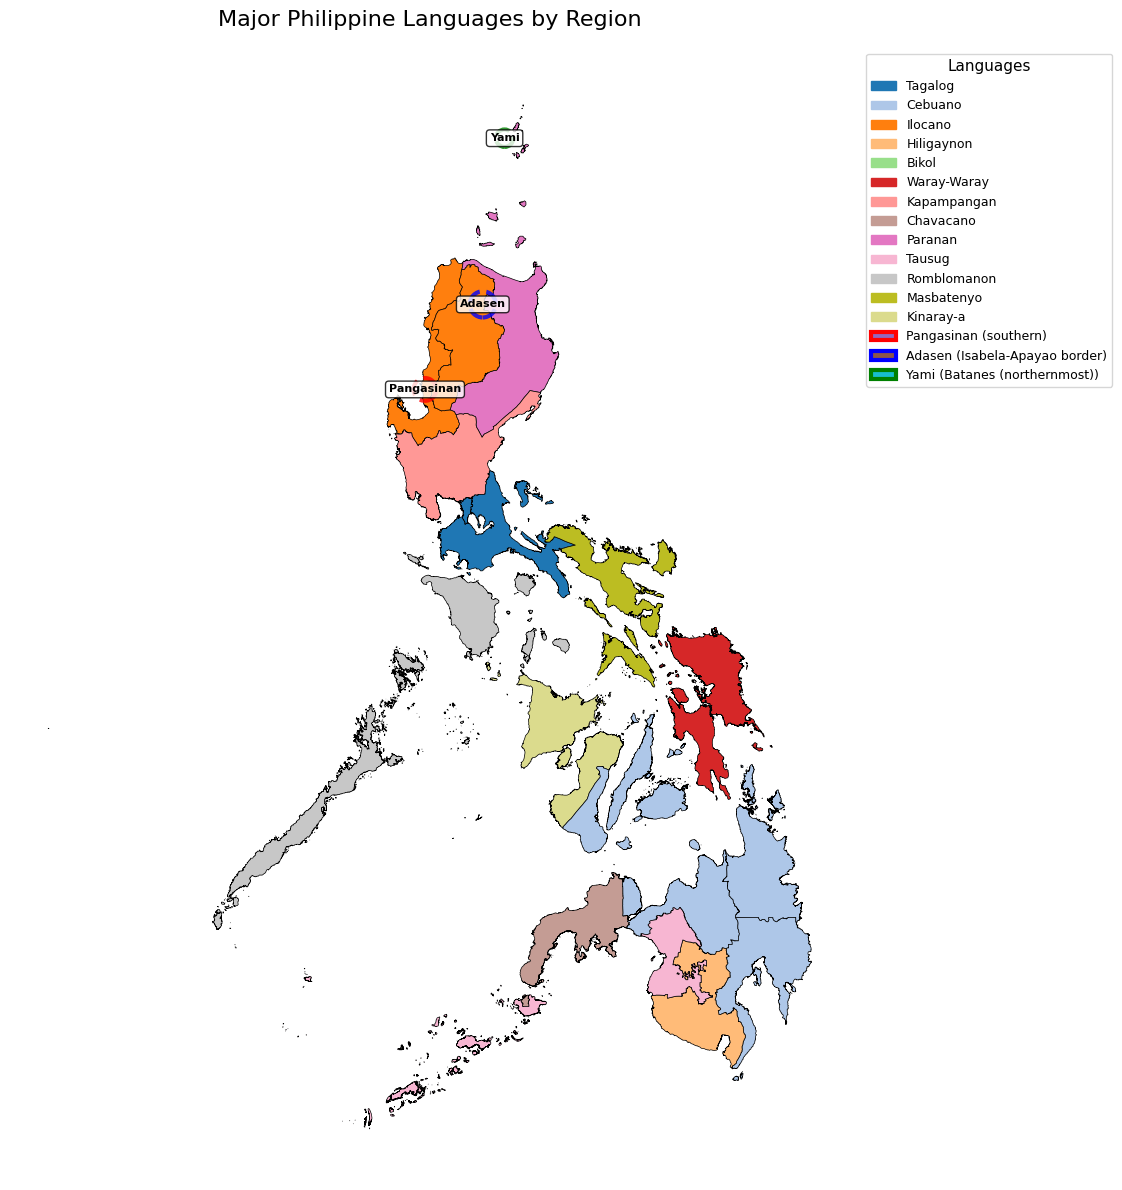
\includegraphics[width=\columnwidth]{chapters/artifacts/lingmap_out.png}
    \caption{Generated linguistic map showing the spatial distribution of the
        selected Philippine languages overlaid on topographic contours. Its
        construction is described in~\cref{sec:geo}.}
    \label{fig:lingmap_out}
\end{figure}
\section{Methodology}

To establish the relationships among the selected languages, we evaluated them
across three dimensions: orthographic, phonetic, and geospatial.

\subsection{Linguistic Distance Metrics}

We extracted unique trigrams from the standardized biblical corpus of each
language to compute two distinct similarity matrices.

First, we measured orthographic similarity using the Jaccard similarity
coefficient, which quantifies the direct overlap of written forms. It is
defined as the intersection of two trigram sets divided by their union:

\begin{equation}
    J(A, B) = \frac{|A \cap B|}{|A \cup B|}
\end{equation}

where \(A\) and \(B\) represent the unique orthographic trigrams for two
languages.

Second, we measured phonetic similarity to capture acoustic properties
independent of spelling conventions. We converted all corpus trigrams into
phonetic representations using the Double Metaphone algorithm, which accounts
for non-English phonological patterns and variant pronunciations. We then
computed the pairwise cosine similarity of these phonetic frequency
distributions:

\begin{equation}
    \text{cos}(\theta) = 
        \frac{\mathbf{A} \cdot \mathbf{B}}{\|\mathbf{A}\| \|\mathbf{B}\|} = 
        \frac{\sum_{i=1}^{n} A_i B_i}{\sqrt{\sum_{i=1}^{n} A_i^2} \sqrt{\sum_{i=1}^{n} B_i^2}}
\end{equation}

where \(\mathbf{A}\) and \(\mathbf{B}\) are the phonetic frequency vectors.
Cosine similarity accounts for the relative distribution of features rather
than absolute frequencies, making it robust to corpus size variations.

\subsection{Geospatial Mapping}

To model how physical terrain influences these linguistic similarities, we
aligned the linguistic data with geospatial boundaries. We sourced language
distribution boundaries from the Komisyon ng Wikang Filipino (KWF)
atlases~\cite{Marrion2025MapaKultural, KWF2025MapaPilipinas} and administrative
data from the UN Office for the Coordination of Humanitarian
Affairs~\cite{OCHA_Philippines_2018_PHL_Admin_Boundaries}. Topographic data
(elevation and hydrology) were obtained from the National Mapping and Resource
Information Authority (NAMRIA)~\cite{NAMRIA_Downloads}. We rendered the
combined digital map using Matplotlib and GeoPandas in
Python~\cite{Hunter:2007, kelsey_jordahl_2020_3946761} to visually and
quantitatively assess the convergence of linguistic boundaries and terrain
discontinuities.
Across the sixteen languages analyzed, orthographic similarity ranges from
0.3423 to 0.9391, while phonetic similarity occupies a much narrower and higher
band (0.7622 to 0.9927). This discrepancy reveals a fundamental dynamic in
Philippine linguistics: spelling has diverged far more rapidly than sound.
Orthography is highly susceptible to external standardization, bearing the
marks of disparate missionary, educational, and administrative decisions even
among neighboring communities. Phonology, by contrast, is markedly more
conservative. The spoken word preserves a shared Austronesian history that
modern spelling conventions obscure. Read against the linguistic map
from~\cref{fig:lingmap_out}, it becomes evident that while
geography—specifically rugged terrain—explains part of this pattern, historical
maritime contact and creolization frequently override geographic boundaries.

\subsection{Visayas and Archipelagic Connectivity}
The Bisayan languages form the most cohesive group in the dataset across both
measures. Rather than acting as barriers, the narrow straits of the Visayas
have functioned as conduits for linguistic exchange. This is most pronounced
between Hiligaynon and Cebuano, which exhibit near-total phonetic convergence
(0.9927) alongside high orthographic similarity (0.9391). Kinaray-a and
Waray-Waray remain closely tied to this core; remarkably, Waray-Waray maintains
a 0.9550 phonetic similarity with Kinaray-a despite being geographically
separated by the Samar Sea.

Romblomanon exemplifies this maritime connectivity. Geographically situated
between the northern and southern migration routes, its linguistic profile
firmly anchors it at the center of the Bisayan cluster rather than its
periphery. It shares high phonetic similarity with Hiligaynon (0.9734), Cebuano
(0.9708), and Tagalog (0.9716), reflecting a historical zone where mutual
intelligibility aligns with the ease of sea travel. Similarly, Bikol and
Masbatenyo form a tight pair (0.9206 orthographically, 0.9857 phonetically),
reflecting their adjacency on the Bicol Peninsula.

Further north, Tagalog pairs closely with Cebuano and Hiligaynon in spelling
(reaching 0.8877 and 0.8811, respectively). This orthographic alignment is
likely sustained by modern educational infrastructure and mass media
standardizing the archipelago's most widely spoken languages, rather than deep
structural convergence.

\subsection{Luzon and the Cordillera Barrier}
In the northern Philippines, physical terrain plays a far more restrictive
role, though the linguistic landscape remains complex. Ilocano demonstrates low
similarity to the central languages in both sound (ranging from 0.76 to 0.79)
and spelling (0.55 to 0.56). This stark division tracks closely with the
Cordillera and Sierra Madre mountain ranges, which have historically isolated
Ilocano speakers from central lowland influences.

However, terrain does not account for all northern variations. Paranan and
Pangasinan display an unexpectedly high phonetic affinity (0.9677) despite
geographic separation, suggesting either the retention of conservative features
lost in central varieties, or parallel trajectories of simplification in
isolated communities. Similarly, Kapampangan proves that geographic adjacency
does not guarantee orthographic convergence. Despite a long literary history in
Central Luzon, its spelling diverges significantly from neighboring Ilocano
(0.5421). Phonetically, however, Kapampangan is closer to the distant Kinaray-a
(0.9456) than to its immediate neighbors. This mismatch characterizes lowland
regions, where historical trade, migration, and urbanization blur the strict
linguistic borders imposed by terrain.

\subsection{The Impact of Creolization}
Chavacano emerges as the clearest outlier in the matrix, demonstrating that
creolization reshapes a language far more aggressively than either distance or
ambient contact. As a Spanish-based creole, its orthographic similarity with
neighboring languages largely bottoms out between 0.35 and 0.45. Phonetically,
it sits near the floor of the dataset, scoring as low as 0.7881 against
Tagalog.

Although Chavacano absorbed extensive vocabulary from Cebuano and Tausug
substrates in Zamboanga, its phonotactics and spelling conventions were
fundamentally reconfigured by Spanish colonizers. The limited orthographic
similarity it does share with other Philippine languages is an artifact of the
shared Latin script, not common ancestry. Its profile firmly suggests that the
mechanics of creolization overwrite inherited Austronesian traits.

\subsection{Summary}
Taken together, these measures demonstrate that phonetic and orthographic data
record two different histories. Orthographic similarity serves as a modern
record of which communities learned to write together under shared
administrative or educational standards. Phonetic similarity offers a deeper,
more conservative record of shared descent and historical contact. Geography
predicts these patterns only where terrain—such as the Cordillera—genuinely
restricts human movement. Where communities could navigate waters, engage in
trade, or experience colonization, human contact readily overwrote the
geographic map. Languages that resist geographic explanation on the phonetic
measure, particularly Yami and Paranan, present clear targets for future
diachronic study.
\section{Conclusion}\label{sec:conclusion}

We measured sixteen Philippine languages across three independent dimensions:
orthography, phonology, and geospatial features. Using trigram-based similarity
matrices and a purpose-built linguistic map. While the two quantitative
matrices agree on the ordering of language relationships, they diverge
significantly in scale, revealing two distinct historical layers. Orthographic
similarity ranges widely (0.3423 to 0.9391), registering colonial-era
standardization at full amplitude. It tracks recent, administratively tractable
histories of missionary, educational, and colonial contact. In contrast,
phonetic similarity operates within a substantially narrower band (0.7622 to
0.9927), preserving a compressed but legible record of shared Austronesian
descent that recent spelling reforms did not erase.

Geography accounts for these patterns where terrain restricted movement, but
fails where it did not; navigable water served to carry contact rather than
block it. Geographically, Romblomanon emerges as central under every measure,
while Northern Luzon forms a distinct zone bounded by the Cordillera and Sierra
Madre, neatly explaining the cohesion of the Bisayan cluster and Ilocano's
separation. Conversely, geography fails to explain Chavacano, which remains
universally peripheral due to creolization rather than physical isolation.
Similarly, geographic models poorly predict the Paranan-Pangasinan affinity,
which owes more to retained older features than to physical terrain.

Ultimately, similarity computed over trigrams cannot separate the retention of
conservative features from convergent innovation or undocumented contact.
Resolving these distinctions requires deeper historical evidence, including
cognate sets, reconstructed proto-forms, and migration histories. The languages
that most resist geographic explanation—foremost Yami and Paranan—are exactly
where this evidence would be most productively sought.


% ACL requires Limitations and (optionally) Ethics Statement as unnumbered
% sections placed after the body and before the references.
\section*{Limitations}
\phantomsection\label{sec:limitations}

The measures employed in this study are deliberately shallow. Orthographic
similarity compares trigram inventories and is therefore sensitive to the
transcription conventions of a particular translation and not solely to the
language that translation transcribes. Phonetic similarity depends upon Double
Metaphone, an encoder developed for English, whose treatment of Philippine
phonology is approximate, uniform across all sixteen languages, and liable to
compress genuine contrasts.

Both measures are computed over Biblical translation, which constitutes a single
register produced by translators working to their own conventions, and eight of
the sixteen corpora cover only the New Testament (\cref{tab:seeds}). Register
and translator effects are consequently confounded with language effects
throughout, and no comparison reported here is able to separate them.

The analysis presented in \cref{tab:metric_comparison} addresses the most
tractable of these concerns, namely corpus size, and establishes that the
disparity in scale between the two measures is not attributable to it. It does
not address the remainder. Those residual concerns bear upon the magnitudes
reported in \cref{sec:synthesis} rather than upon the ordering of language
relationships, and it is upon the ordering that the convergent findings of that
section principally rest.

\section*{Ethics Statement}
\phantomsection\label{sec:ethics_stmt}

The corpus underlying this paper was obtained by automated retrieval from
YouVersion (\url{https://www.bible.com}) in September 2025. We reviewed the
instruments governing automated access to that site after collection rather than
before it, and report the outcome plainly here.

The crawl conformed to the site's robots exclusion file. It did not conform to
the site's Terms of Use, which prohibit the use of ``any robot, spider, or other
automatic device, process, or means'' to access YouVersion or copy material from
it. We do not claim compliance with that clause: our crawler is the conduct it
names. The collection was non-commercial, circumvented no access control, and
identified itself as an automated agent rather than imitating a browser, but we
offer these as mitigation and not as a cure.

The translations are separately the copyright of their publishers, and no
verbatim verse text is released from this project. The similarity matrices
reported above are derived statistics from which the source cannot be
reconstituted, and are the appropriate unit of release. YouVersion's Platform API
offers a sanctioned route, and any continuation of this work should re-collect
through it.


\bibliography{refs}

\appendix
\crefalias{section}{appendix}
\crefalias{subsection}{appendix}
\section{Data Collection}\label{sec:data_collection}

The orthographic and phonetic analyses in this paper are computed over a corpus
of Biblical translations that we collected ourselves. Because that corpus is
unpublished, its provenance cannot be established by citation, and we therefore
document the collection procedure here in full rather than referring the reader
elsewhere.

\subsection{Source and Procedure}

The corpus was drawn from YouVersion (\url{https://www.bible.com}), an online
Bible platform that hosts translations under license from their publishers. One
translation was selected per language for each of the sixteen languages
in~\cref{tab:ph_languages}. \Cref{tab:seeds} records the exact translation used
for each, together with the number of chapters obtained from it. Eight of the
translations are complete Bibles and were seeded at Genesis 1. The remaining
eight are New Testament translations still in progress and were seeded at
Matthew 1, which is why their chapter counts are uniformly lower.

\begin{table}[h!]
    \centering
    \footnotesize
    \begin{tabular}{llr}
        \hline
        \textbf{Language} & \textbf{Seed chapter}        & \textbf{Chapters} \\
        \hline
        Tagalog           & \texttt{2195/GEN.1.ABTAG01}  & 977               \\
        Cebuano           & \texttt{562/GEN.1.RCPV}      & 977               \\
        Ilocano           & \texttt{782/GEN.1.RIPV}      & 977               \\
        Hiligaynon        & \texttt{2190/GEN.1.MBBHIL12} & 1{,}104           \\
        Bikol             & \texttt{890/GEN.1.MBBBIK92}  & 1{,}104           \\
        Waray-Waray       & \texttt{2198/GEN.1.MBBSAM}   & 1{,}104           \\
        Kapampangan       & \texttt{1141/GEN.1.PMPV}     & 1{,}104           \\
        Pangasinan        & \texttt{1166/GEN.1.PNPV}     & 1{,}104           \\
        Adasen            & \texttt{2812/MAT.1.YBT}      & 209               \\
        Chavacano         & \texttt{1129/MAT.1.CBKNT}    & 209               \\
        Paranan           & \texttt{438/MAT.1.PRF}       & 209               \\
        Tausug            & \texttt{1319/MAT.1.TSG}      & 209               \\
        Romblomanon       & \texttt{2244/MAT.1.BKR}      & 209               \\
        Masbatenyo        & \texttt{1222/MAT.1.MSB}      & 209               \\
        Kinaray-a         & \texttt{1489/MAT.1.KRJNT}    & 209               \\
        Yami              & \texttt{2364/MAT.1.SNT}      & 209               \\
        \hline
                          & \textbf{Total}               & \textbf{10{,}123} \\
        \hline
    \end{tabular}
    \caption{Seed chapter and yield per language. Each seed is given relative to
        the prefix \url{https://www.bible.com/bible/}.}\label{tab:seeds}
\end{table}

YouVersion serves each chapter as an HTML document in which every span whose
class is prefixed with \texttt{ChapterContent\_verse\_\_} encloses one verse.
Within such a span, the verse text is carried by descendants prefixed
\texttt{ChapterContent\_content\_\_}, while editorial apparatus supplied by the
platform rather than by the translators, such as footnotes and
cross-references, occupies \texttt{ChapterContent\_note\_\_} descendants
interleaved with the text. We retained only the \texttt{content} descendants,
concatenated in document order, and discarded every sibling class. The corpus
consequently contains the translated text alone, and no editorial contribution
of YouVersion's own. Each chapter page also carries a navigation anchor to its
successor, which the collector followed from the seed, so each translation was
traversed as a linear chain rather than as a general crawl of the site.

Collection was performed once, in September 2025, using a purpose-written
crawler in Go built on the Colly framework. Traversal from each seed terminated
when the next-chapter link was exhausted rather than at the configured ceiling
of 30,000 chapters, which was never binding. Each language was collected in its
own goroutine, giving sixteen
concurrent request streams, and the implementation issued two requests per
chapter, one to extract the verses and a second to resolve the next-chapter
link. The sixteen streams together therefore placed on the order of 20,000
requests on the host. No crawl delay or rate limit was configured. The crawler
transmitted Colly's default user agent, which identifies the client as an
automated agent rather than imitating a browser.

Only pages that YouVersion serves publicly and anonymously were retrieved. The
crawler held no account, transmitted no credentials, and circumvented no
paywall, login, or other access control; it read the same markup that the site
returns to any unauthenticated visitor.

\section{Ethical Considerations}\label{sec:ethics}

Because the corpus underlying this paper was collected from a third party's
website rather than obtained from a published dataset, the procedure
of~\cref{sec:data_collection} requires scrutiny against the two instruments that
govern automated access to that site: its robots exclusion file and its Terms of
Use. We reviewed both, and we report the outcome in full, including where it is
unfavorable to us.

\subsection{Robots Exclusion}

At the time of review, the robots exclusion file at
\url{https://www.bible.com/robots.txt} applied a single rule set to all user
agents. It disallows \texttt{/bible/*/*/notes}, the user and plan search
endpoints, and five language-code directories, and it specifies no
\texttt{Crawl-delay}. The chapter pages we retrieved lie under \texttt{/bible/}
but match none of the disallowed patterns, and no disallowed path was requested.
The crawl therefore conformed to the robots exclusion file.

This conformance was, however, incidental rather than enforced. The Colly
collector sets its \texttt{IgnoreRobotsTxt} option to true on construction and
our implementation did not override it, so the crawler never retrieved or
evaluated the exclusion file at run time. Conformance was established by our own
later inspection, not by the software: had the file disallowed \texttt{/bible/},
the crawler would have proceeded regardless. We record this because a claim of
conformance that rests on coincidence is weaker than one that rests on
enforcement, and the reader is entitled to the distinction.

\subsection{Terms of Use}

The YouVersion Terms of Use are less permissive than the exclusion file. Under
the heading ``Permitted and Unpermitted Use'' they prohibit the user from

\begin{quote}
    ``us[ing] any robot, spider, or other automatic device, process, or means to
    access YouVersion for any purpose, including monitoring or copying any of the
    material on YouVersion''.
\end{quote}

We do not claim that our collection complies with this clause. It does not. The
crawler described in~\cref{sec:data_collection} is an automatic device that
accessed YouVersion for the purpose of copying material from it, which is the
conduct the clause names. A permissive robots exclusion file does not cure this,
as the two instruments are independent and the Terms are the governing agreement
between the site and its users. The order of events is likewise material and we
state it plainly: collection was carried out in September 2025, and the review
reported here was conducted afterwards. The Terms were not consulted before the
corpus was obtained, and the question was settled after the fact rather than in
advance.

We disclose this rather than assert a compliance we do not have. So that the
reader may weigh the matter independently, we set out the circumstances on both
sides.

Four circumstances mitigate. The use is non-commercial and academic, and no
revenue is derived from the corpus or from any work built upon it. No technical
protection measure was defeated: every page retrieved is served publicly and
anonymously, and the crawler bypassed no paywall, login, or access control. The
crawler identified itself honestly rather than imitating a browser, so its
automated character was apparent in the host's request log and was never
disguised. The collection was a single bounded pass rather than a standing
service, and nothing continues to poll the site.

Three circumstances aggravate, and we do not minimize them. No crawl delay was
configured, so requests were issued as fast as the parser allowed rather than at
a rate calibrated to the host's capacity. Sixteen concurrent streams ran
simultaneously. The implementation fetched each chapter twice, once for its
verses and once for its next-chapter link, which doubled our load on the host
for no benefit to us and could have been avoided by resolving both from a single
response. The approximately 20,000 requests we placed were thus roughly twice as
many as the task required, delivered without pacing. A defensible crawl would
have used one request per chapter, a fixed delay, and a single stream.

\subsection{Remediation}

The defect identified here is remediable, and the remedy is specific. YouVersion
operates a Platform API at \url{https://developers.youversion.com} which provides
programmatic access to its Bible collections under a developer agreement, at no
cost, and with a non-commercial restriction that an academic project satisfies by
construction. It covers substantially more versions and languages than the
sixteen used here. Obtaining the corpus through that interface would place the
collection within the terms the site sets for automated access, and would
dissolve the conflict described above rather than merely mitigate it. We
recommend that any continuation of this work re-collect through the Platform API,
and that the present corpus be treated as provisional until it does.


\end{document}
